As already mentioned earlier, the \textit{data capture} process is split into two parts.\\
The first part is the evaluation of a survey handed to the management of the company, i.e. the \textit{company provided data}. This first part can be implemented via a survey that is being transmitted to us.\\
The second part of \textit{data capture}, the \textit{employee survey}, is a special point of interest. Because it is important to guarantee anonymity to the employee and at the same time ensure validity and transparency of the data that is provided. We implemented this second part with a protocol that is equivalent to an \textit{E-voting system} that is explained in detail below.\\

\paragraph*{E-voting protocol}
A company that wants to be part of our rating applies and sends their unverified data via smart contract (contract \texttt{SurveyFactory}) to the blockchain. This initiates the whole process of survey generation.
\begin{lstlisting}
// https://github.com/EriCreator/bEquality/blob/master/Survey.sol
/*	SurveyFactory serves as a hub 
	(deployed on the blockchain upon the launching of bEquality)
	Company can create their own survey by providing a list of permitted user address. */

contract SurveyFactory {

  //address owner;
  mapping(uint => address) public SurveyContracts;

  // function SurveyFactory(address adr) public 
  // {
  //		owner = adr;
  // }

  function createNewSurvey(uint companyID, address[] addressessOfEmployees, string _hashToaddressessOfEmployees) public returns(address newContract)
  {
    // require(msg.sender == owner);
    require(SurveyContracts[companyID] == 0x0);
    Survey c = new Survey(addressessOfEmployees, _hashToaddressessOfEmployees);
    SurveyContracts[companyID] = c;
    return c;
  }
  
  function getContractAddress(uint companyID) public constant returns (address)
  {
    return SurveyContracts[companyID];
  }
}
\end{lstlisting}
They also send bEquality the email addresses of all emplyees, as observable in the function \texttt{createNewSurvey}), which we store in a secure and private data base.\\
We do not store the password of the employee explicitly, we instead store the hashed password linked to the corresponding username. To further link the private key to the account, we also store the hashed private key on our database.\\
This account stored on our database does not allow us to login to the user-account, but we can verify validity of the account, when a user wants to log in.
\begin{figure}[H]
	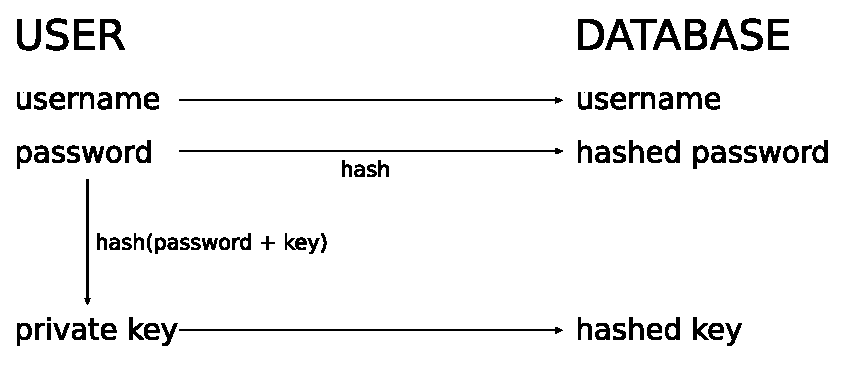
\includegraphics[width=0.6\textwidth]{Bilder/SecureLoginDataStorage-scheme.eps}
	\caption{Secure login data storage}
	\label{Secure_Login_data_storage}
\end{figure}
\comment{Is this correct?}
When all accounts are set up and put money on them to pay for the transaction costs, the employee gets notified that he has to log into his account and fill out the survey.\\
The employee then acts on the following smart contract \texttt{Survey}, that only he can modify, but not the contract-creator.\\
When the employee has filled out his survey, he submits his data via a user-friendly interface and the data gets stored anonymously on the blockchain. The user therefore can verify that his data is not altered, but at the same time there is guaranteed that the employer cannot prosecute the employee for telling the truth about the company.

\begin{lstlisting}
// https://github.com/EriCreator/bEquality/blob/master/Survey.sol
/*
   Survey is the child contract created by the SurveyFactory where only the permitted user can modify.
*/

contract Survey {
    mapping (address => string) public hashes;
    mapping (address => bool) public isAllowedToSumbitSurvey;
    string hashToaddressessOfEmployees;

    function Survey(address[] addressessOfEmployees, string _hashToaddressessOfEmployees) public {
        hashToaddressessOfEmployees = _hashToaddressessOfEmployees;
        for (uint256 index = 0; index < addressessOfEmployees.length; index++) {
            isAllowedToSumbitSurvey[addressessOfEmployees[index]] = true;
        }
    }

    function submitResults(string myHash) public {
        require(bytes(hashes[msg.sender]).length == 0);
        require(isAllowedToSumbitSurvey[msg.sender]);
        hashes[msg.sender] = myHash;
    }

}
\end{lstlisting}


Because all data is stored on the blockchain, everyone can verify the integrity of our analysis, and can even make his own analysis of the given data. This allows full transparency towards the shareholders and future investors in the company.\\

Yet there are still challenges ahead of us, for example the possibility of storing the Ethereum addresses on the blockchain instead of a private database for further transparency and automation of the process.\\

Below is shown the full protocol in a schematic way, to give the reader an overeview of our E-voting protocol.
\begin{figure}[H]
	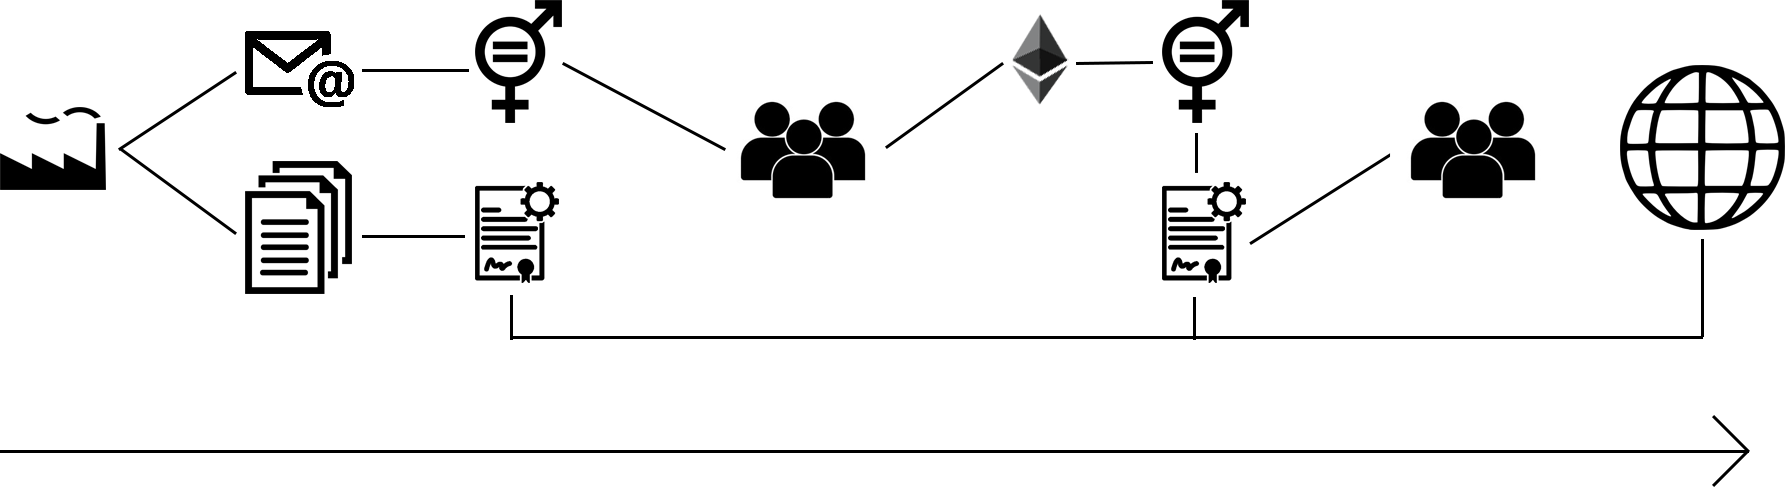
\includegraphics[width=0.9\textwidth]{Bilder/Survey_Protocol_preview_2}
	\caption{technical flow representation of the data capture and storage process}
	\label{technical_flow_representation}
\end{figure}

\comment{CANCEL THAT?? (below):
\paragraph*{Survey for Employer}
The survey handed to the employer, that applies to our gender-equality index, is based on already existing frameworkds such as the Bloomberg gender-equality index or the gender-equality index of Equileap.\\

-based on existing frameworks such as Bloomberg, Equileap\\
capturing data with app or web
-delivers e-mail addresses from employees\\
--addresses stored on private database\\
-survey stored on IPFS\\
-explain interaction with web/App 
}

We now dive deeper into details of the implementation of the employee survey.


\paragraph*{Survey for Employees}
The survey for the employees presents the employee with gender specific questions and also with questions applicable for both men and women. These questions guarantee further insight into the microclimate of the employees that cannot be obtained by just consulting the company management.\\

We earlier explained that we hand our survey to just a randomly chosen percentage of all employees. This is done to increase efficiency of the gender-equality index while cutting costs of applying to that index. The random sample provides us with a hopefully real view of the microclimate of employees. Unfortunately this random sample could lead to a completely wrong picture of the company, we therefore have the option to increase this sample, when there is too much variation from the employer provided data.\\

\paragraph*{capturing data with app}
To make the survey as easy as possible for the employees, we came up with providing an app for this task. We build an example app for android smartphones with the android studio IDE.
Our app is only a placeholder for an actual implementation. That means, that our example app consists of a sample survey and dummy buttons (app can't submit survey).
Because of the limited time, we couldn't build a working app. Besides the time factor, we didn't know how to link the app with the Blockchain/IPFS and if there is even a java Interface to accomplish this task. 
Nevertheless our app is just an example, how a survey app can look like.\\

(--insert pictures of the app--)

The fully implemented app could then work as follows: 1. The employee sees a login screen and is asked to fill in his e-mail address and his password.
2. After the login was successful, the app shows it's user the questions to answer. The interface to answer the questions is straightforward and self explanatory. 
3. After the user submits the survey, the app sends the Survey to the Blockchain/IPFS and reports that the submission was successfull. 
The big advantage of an app is the self explanatory user interface. But there are also disadvatages of an app. Some of them are: 1. even for one survey, the app needs to be installed. 2. Survey questions are hardcodeed in the current app. \\
The second problem can be solved, such that the app downloads the survey questions, after the user is logged in. With this approach the app serves as a framework for all kinds of surveys. \\
To conclude, we can say, that the app can exploit it's advantages, if the employee needs to answer more than one query in shorter periods. For a gender equality survey, this might not be the case, but we can easy deduce other use cases which needs several queries.\\

\comment{
capturing data with app or web\\
-explain,that process automated in the background\\
-what does the employee has to do\\
-what is done behind the scenes
}


\comment{	
storing data: blockchain, IPFS, (some on server)\\
-how is privacy of data secured\\
-explain process, what does this mean for different data\\
--sensibele data -- server\\
--insensible data -- ipfs\\
--non-fakeable -- blockchain\\
-explain cost aspect of storing stuff on blockchain or on IPFS (storing on blockchain costly)
}

\comment{
how can anonymity/privacy be ensured\\
-because data on blockchain, IPFS, it is visible for everybody, but boss should not be able to track the results of employees (how do we solve that)\\

state technical problems
}

